\chapter{Big Chapter Title}


\chaptermark{Short Chapter Title}





\section{Introduction}
\lipsum[1-2]
\begin{equation}
    \frac{\left( {{1}\Bigg/{\sqrt{2\pi \sigma _{0}^{2}}}} \right) ^n\exp \left\{ {{\left( -\sum_{i=1}^n{\left( x_i-\mu _0 \right) ^2} \right)}\Bigg/{2\sigma _{0}^{2}}} \right\}}{\left\{ {{1}\Bigg/{\left( \frac{2\pi}{n} \right) \sum_{i=1}^n{\left( x_i-\mu _0 \right) ^2}}} \right\} ^{\frac{n}{2}}e^{-\frac{n}{2}}}
\end{equation}


\section{Automatic A+ Maker Model}

\lipsum[1-2]
\begin{figure}
    \centering
    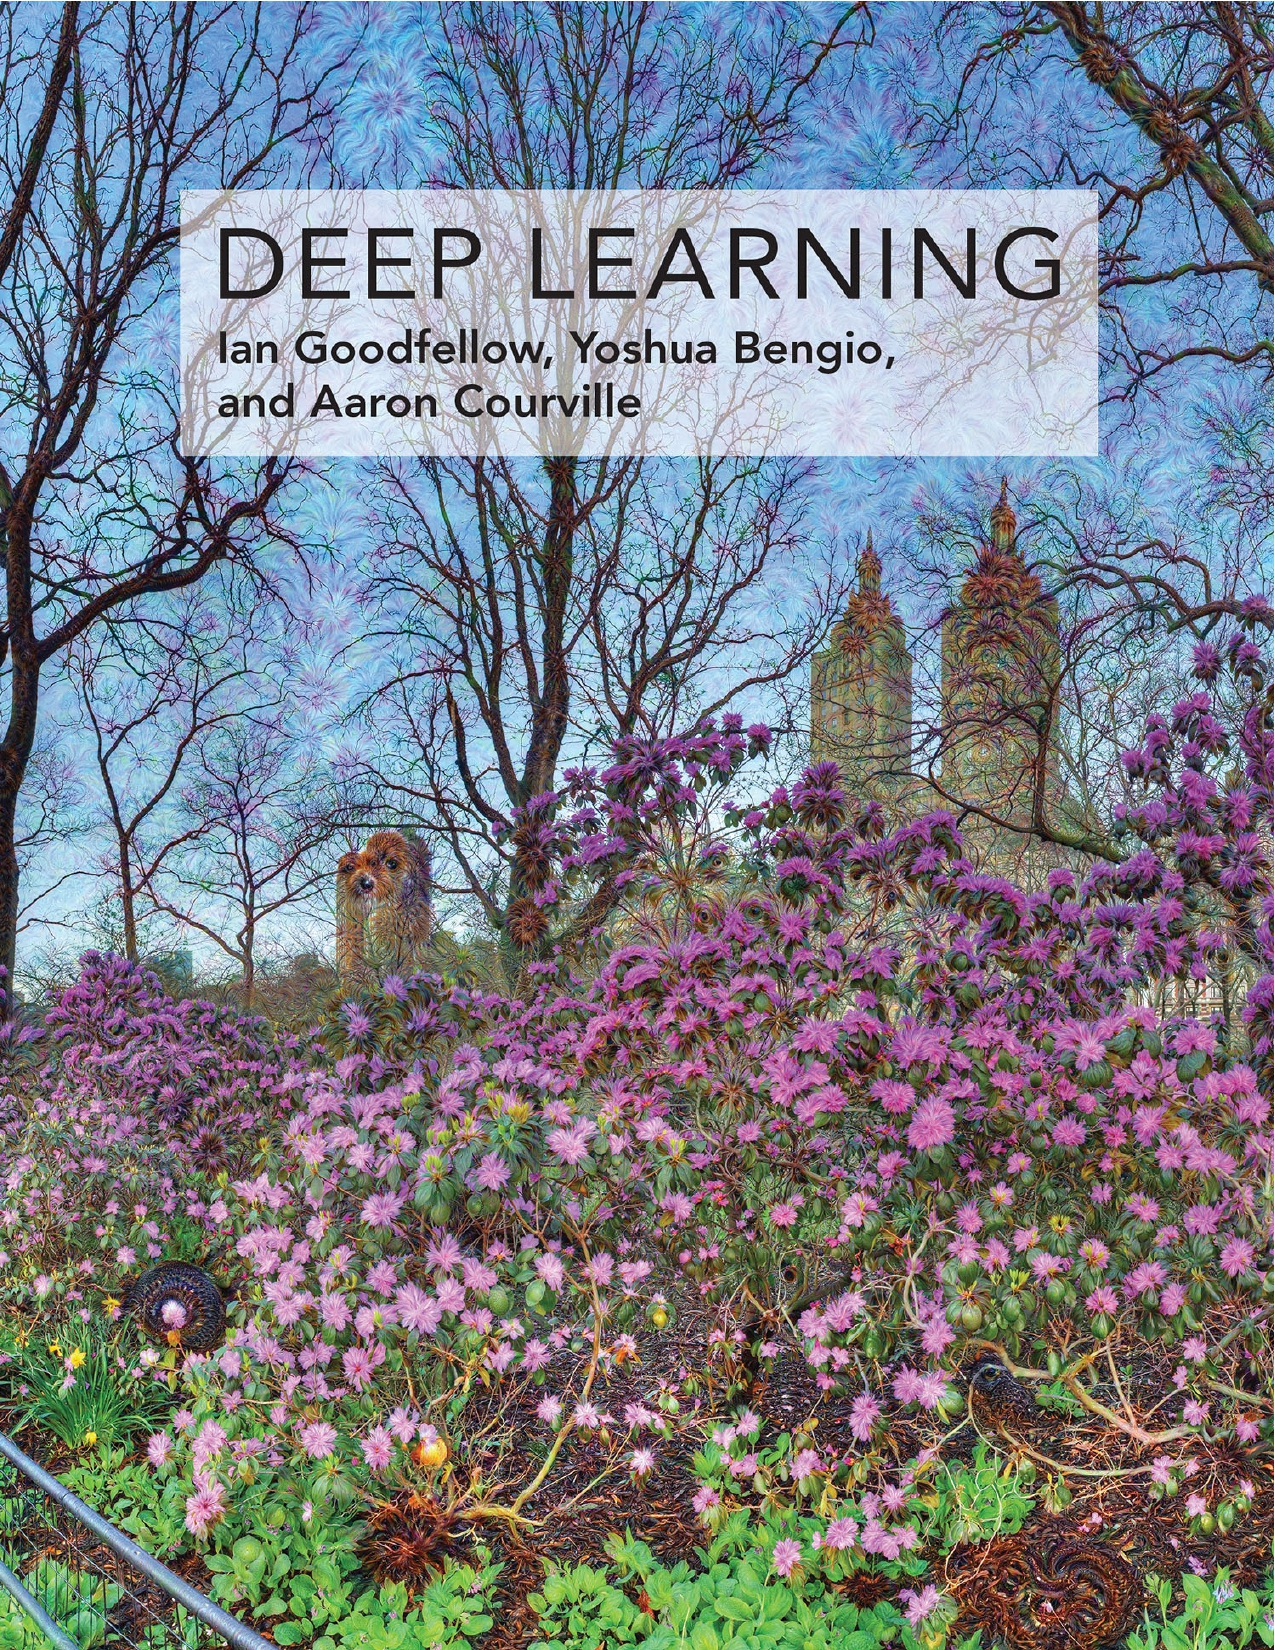
\includegraphics[width=8cm]{pic/DeepLearning.jpg}
\end{figure}
\lipsum[1-2]

\begin{equation}
    \left\{ \begin{array}{l}
        \nabla \cdot \boldsymbol{E}=\frac{\rho}{\varepsilon _0}\\
        \nabla \times \boldsymbol{E}=-\frac{\partial \boldsymbol{B}}{\partial t}\\
        \nabla \cdot \boldsymbol{B}=0\\
        c^2\nabla \times \boldsymbol{B}=\frac{\boldsymbol{j}}{\varepsilon _0}+\frac{\partial \boldsymbol{E}}{\partial t}c^2\\
    \end{array} \right. 
\end{equation}



\begin{equation}
    \left\{ \begin{array}{l}
        \oiint_{\partial \Omega}{\boldsymbol{E}\cdot \mathrm{d}s}=\frac{Q}{\varepsilon _0}\\
        \oiint_{\partial \Omega}{\boldsymbol{B}\cdot \mathrm{d}s}=0\\
        \oint_{\partial \Omega}{\boldsymbol{E}\cdot \mathrm{d}\ell}=-\frac{\mathrm{d}\varPhi _B}{\mathrm{d}t}\\
        \oint_{\partial \Sigma}{\boldsymbol{B}\cdot \mathrm{d}\ell}=\mu _0I+\mu _0\varepsilon _0\frac{\mathrm{d}\varPhi _E}{\mathrm{d}t}\\
    \end{array} \right.
\end{equation}



\subsection{Super humam practice finisher}

\lipsum[1-2]

\section{Conclusions}
\lipsum[1-5]
This is the conclusion part of the paper body. 